\documentclass[12pt, twoside]{article}
\usepackage[letterpaper, margin=1in, headsep=0.5in]{geometry}
\usepackage[english]{babel}
\usepackage[utf8]{inputenc}
\usepackage{amsmath}
\usepackage{amsfonts}
\usepackage{amssymb}
\usepackage{tikz}
%\usetikzlibrary{quotes, angles}

\usepackage{graphicx}
\usepackage{enumitem}
\usepackage{multicol}

\usepackage{fancyhdr}
\pagestyle{fancy}
\fancyhf{}
\renewcommand{\headrulewidth}{0pt} % disable the underline of the header

\fancyhead[RE]{\thepage}
\fancyhead[RO]{\thepage \\ Name: \hspace{3cm}}
\fancyhead[L]{BECA / Dr. Huson / 10th Grade Geometry\\* 11 January 2019}

\begin{document}
\subsubsection*{Homework: Regents exploration, due Monday}

Use the last four digits of your student number as your Gradecam ID. Write the number and bubble in your ID (1 point).\\[0.5cm]
Review the whole test first, circling the questions you are most certain of.\\[0.5cm]
\textbf{Multiple Choice: } Answer 6 multiple choice questions in the grade cam bubbles. Complete up to three additional multiple choice problems below (spicy).\\[0.5cm]
\textbf{Free Response: } Complete 6 free response questions in that section of the test. \\[0.5cm]

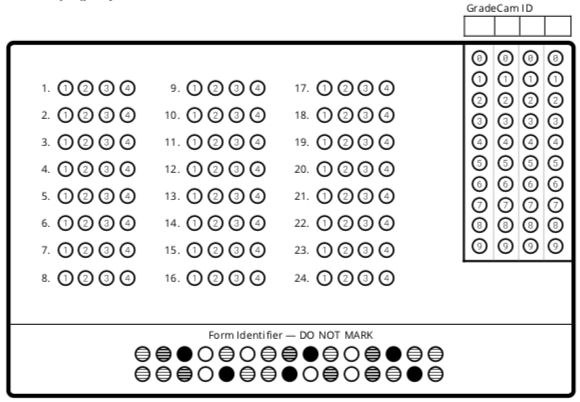
\includegraphics[width=0.7\textwidth]{gradecam-24.png} \\ \vspace{0.5cm}
Answer up to 3 additional multiple choice problems below. (spicy)


\end{document}
